\chapter{Spectrum-efficient Pilot-based CSI Feedback}
\label{chap:p2d}

This chapter details a scheme for acquiring angular-delay domain CSI at the UE based on a limited number of spatial-frequency domain pilots. This scheme adheres to the 3GPP standard for pilot allocation across time-frequency resources.

\section{Sparse Pilots in Practical Networks}

To estimate the downlink CSI in wireless networks, transmitters allocate pilot reference signals. To reserve spectral resources, pilots are restricted to a limited number of spatial-frequency positions, and the allocation of these pilots is defined in the 3GPP technical standards, TS 36.211 for 4G/LTE networks \cite{ref:3gpp.36.211} and TS 38.211 for 5G/NR networks \cite{ref:3GPPTS38.211V15.8.0}. In these two standards, the pilots are called CSI reference signals (CSI-RS) or demodulation reference signals (DM-RS), respectively. Figure~\ref{fig:lte-vs-5g} shows valid placements of CSI-RS/DM-RS in the time-frequency resource grid as defined by TS 36.211 and TS 38.211.

\begin{figure}[!hbtp]
    \centering
    \includegraphics[width=\linewidth]{LTE_vs_5GNR_resource_grid.png}
    \caption{(a) LTE resource blocks with CSI-RS locations. (b) 5G NR resource blocks with DM-RS locations.}
    \label{fig:lte-vs-5g}
\end{figure}

Considering the sparse placement pilot is important for practical deployment of CSI estimation networks. The works discussed thus far have assumed that (truncated) angular-delay domain CSI is readily available at the UE. However, the pilots as defined in 3GPP standards are defined in the spatial-frequency domain, and to utilize these pilots effectively with CSI estimation networks, one must specify a method for estimating the delay-domain CSI based on the sparse pilots. 

The following section details the pilots-to-delay estimator (P2DE), and Figure~\ref{fig:p2d} demonstrates the operating principle behind P2DE. 

\begin{figure}[!hbtp]
    \centering
    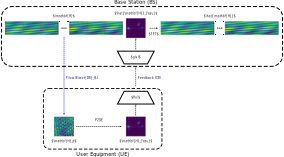
\includegraphics[width=\linewidth]{./images/00_downlink_p2d_feedback_horiz_diag.png}
    % \input{figure/csinet_quant.pdf_tex}
    \caption{Compressive CSI estimation based on linear P2D estimator. First,
    we use downlink pilots to 
    generate a sparse, frequency domain CSI
    estimate 
    of size $M_f << N_f$. We then apply
    the P2D estimator, $\mathbf{Q}^\dag_{N_t}$ of (\ref{eq:p2d_short}), to establish 
    the truncated
    delay domain CSI estimate.
    We train a
    learnable encoder, 
    $f(x)$,
    and decoder, $g(x)$, to compress and decode the feedback, respectively. The 
    gNB recovers
    the frequency domain
    CSI from 
    the decoded 
    delay domain CSI estimate.}
    \label{fig:p2d}
\end{figure}

\section{Pilots-to-delay Estimator (P2DE)}

Denote $\boldeta_i \in \mathbb{C}^{N_f}$ as the $i$-th row of the spatial-frequency matrix $\mathbf{H}$, and denote the downsampled version of $\boldeta_i$ as $\boldeta_{d,i} \in \mathbb{C}^{M_f}$ where $M_f << N_f$. Thus, the spatial-frequency CSI, $\mathbf{H}$, and its downsampled counterpart, $\mathbf{H}_d$, can be written as,
\begin{equation}
	\mathbf{H} = \begin{bmatrix} \boldeta_1 \\ \boldeta_2 \\ \vdots \\ \boldeta_{N_b} \\\end{bmatrix}\in\mathbb{C}^{N_b \times N_f}, \; \mathbf{H}_d = \begin{bmatrix} \boldeta_{d,1} \\ \boldeta_{d,2} \\ \vdots \\ \boldeta_{d,N_b} \\\end{bmatrix}\in\mathbb{C}^{N_b \times M_f}.
\end{equation}
$\boldeta_{d,i}$ is related to $\boldeta_i$ by the downsampling matrix for the $i$-th antenna port, $\mathbf{P}_i$, as
\begin{equation}
	\boldeta_{d,i} = \boldeta_i \mathbf{P}_i \; \forall \; i \in [1, \dots, N_b].
\end{equation}
Denote the delay-domain CSI vector, $\tilde{\boldeta}_i$, which is defined as
\begin{equation}
	\tilde{\boldeta}_{i}\mathbf{F} = \boldeta_i, \label{eq:dft}
\end{equation}
where $\mathbf{F}$ is the $\mathbf{C}^{N_f \times N_f}$ discrete Fourier transform (DFT) matrix. To relate the frequency domain pilots to the delay domain, we apply the pilot downsampling matrix $\mathbf{P}_i$ to both sides of \ref{eq:dft},
\begin{align}
	\tilde{\boldeta}_{i}\mathbf{F}\mathbf{P}_i = \boldeta_i\mathbf{P}_i \nonumber \\
	\tilde{\boldeta}_{i}\mathbf{Q}_i = \boldeta_{d,i} \label{eq:qmat}
\end{align}
where $\mathbf{Q}_i=\mathbf{F}\mathbf{P}_i\in\mathbb{C}^{N_f\times M_f}$ is the downsampled DFT matrix.
Leveraging the sparsity of CSI data in the delay domain (see Section~\ref{sect:sparse-csi}, Figure~\ref{fig:freq-vs-delay}), many works choose to feedback and compress the truncated delay domain vectors, $\tilde{\boldeta}_{c,i}\in\mathbb{C}^{N_t}$. The zero-padded vector $\tilde{\boldeta}_{i}$ defined as
\begin{align*} 
	\tilde{\boldeta}_{i} = \left[\tilde{\boldeta}_{c,i}, \mathbf{0}_{N_f - N_t}\right].
\end{align*}

Based on \ref{eq:qmat}, the delay domain can be related directly to the pilots by taking the pseudoinverse,
\begin{align}
	\tilde{\boldeta}_{i}\mathbf{Q}_i\mathbf{Q}_i^T &= \boldeta_{d,i}\mathbf{Q}_i^T \nonumber \\
	\tilde{\boldeta}_{i} &= \boldeta_{d,i}\mathbf{Q}_i^T\left(\mathbf{Q}_i\mathbf{Q}_i^T\right)^{-1} \nonumber \\
	&= \boldeta_{d,i}\mathbf{Q}_i^{\#} \label{eq:p2d}
\end{align}

\begin{figure}[!hbtp]
    \centering
    \includegraphics[width=\linewidth]{./images/01_p2d_pilots_diag_with_resource_grid.png}
    % \input{figure/csinet_quant.pdf_tex}
    \caption{(a) LTE Resource Blocks and CSI-RS locations where antenna port pilots are allocated. (b) Schematic for diagonal pilots with relevant parameters, size of diagonal $D$ and frequency downsampling ratio $\text{DR}_f$. In this diagram, $N_b=32, D=4, \text{DR}_f=\frac 18$. The pilot matrix $\mathbf{P}_j$ indicates the downsampling pattern for the $j$-th element of the diagonal pattern. The number of subframes necessary to populate (b) is inversely proportional to $D$.}
    \label{fig:p2d_diag}
\end{figure}

\subsection{Results}

\lipsum[1-3]
